\documentclass[journal]{IEEEtran}

\usepackage{algpseudocode}
\usepackage{verbatim}
\usepackage{pgfplots}
\usepackage{float}

%\ifCLASSINFOpdf

%\else

%\fi

%\hyphenation{}

\begin{document}
\title{Applications and Optimizations of Parallel Programming}

\author{\IEEEauthorblockN{Thomas Eubank\\thomas.eubank516@gmail.com\\}\IEEEauthorblockA{Computer Science Department\\ Morehead State University \\}}

\maketitle

\begin{abstract}
\par This project explores the performance benefits of parallel programming across two related problems: matrix multiplication and neural network training. For matrix multiplication, several SYCL-based optimization strategies were evaluated on a Ryzen 5 9600X, comparing CPU buffer and Unified Shared Memory allocations, loop parallel decomposition, and kernel organization. The SYCL USM implementation achieved a median runtime of 0.046 seconds multiplying two 1000x1000 matrices, compared to 0.142 seconds for a 12-thread OpenMP baseline — more than three times speedup without tiling or vendor-specific tuning. The key finding was that outer-loop parallelism outperformed fine-grained strategies, and that memory model selection had the largest single impact on performance.
\par These findings directly informed the design of a standalone C++ neural network API built as the applied contribution of this project. Rather than parallelizing inside individual matrix operations, the API distributes work at the batch level, assigning each thread a complete forward pass over a sample. Benchmarked on the UCI thyroid dataset, this approach reduced training time by approximately 44\% at two threads: with even more speedups with added threads. The result confirms the central thesis: workload size must determine parallel decomposition. The same fine-grained strategies that hurt matrix multiplication performance at small scale hurt neural network performance for the same reason. The API is designed with modular backend classes, leaving a clear path toward GPU acceleration and broader device portability as future work.
\end{abstract}

\begin{IEEEkeywords}
OneAPI, SYCL, GPU Programming, Matrix Multiplication, Parallel Computing, Neural Network, OpenMP
\end{IEEEkeywords}

\section{Introduction}
\IEEEPARstart{G}{PUs} have become one of the most important components in modern high performance computing (HPC), enabling large-scale parallelism for simulation, machine learning, graphics processing, and more being explored 'concurrently'. 
\par Particle simulations, for instance, not only improve the visuals of video games but make weather modeling more effective — resulting in earlier advance notice of natural disasters including hurricanes and tornadoes. The same principles apply to earthquake and landslide damage prediction by modeling how soil interacts under extreme circumstances. At the systems level, the growth of the internet has created pressure on server infrastructure, driving the adoption of container orchestration technologies like Kubernetes that distribute workloads across parallel server architectures. General purpose robotics represent another emerging application, where individual threads for each sensor stream are a hard requirement for maintaining stability in dynamic environments. These are not future possibilities — they are active areas of development where parallel programming is already saving lives and shaping infrastructure. However, developers increasingly need tools to utilize GPUs to their full potential, especially given that a single GPU can cost thousands of dollars.
\par While many tools exist to help developers program GPUs, writing highly portable and optimized GPU code remains a challenge due to the diversity of vendor specific frameworks such as CUDA, HIP, and ROCm. However, there are many open frameworks, including Intel's SYCL parallel programming model, that are designed to be compatible with multiple GPU vendors. 
\par The difficulty of writing parallel programs is compounded when considering the computational demands of neural network training. Matrix multiplication is the primary operation in forward and backward passes, making it one of the most performance-critical operations in machine learning. As such, applying the optimizations achieved through parallel programming to this task is a natural extension of this work. 
\par So, to demonstrate the importance of Parallel Programming, this project explores some of the many Applications and Optimizations of Parallel Programming by analyzing performance and portability, culminating in the development of a standalone neural network API in C++.

\section{Related Works}
\par Several studies have evaluated the performance and portability of SYCL across heterogeneous hardware, providing important context for the results presented in this work. Johnson et al. conducted a broad evaluation of contemporary SYCL implementations across multiple GPU vendors and benchmark kernels, finding that performance varied significantly depending on the implementation and target hardware. [5] Their results highlight that portability does not come for free; achieving competitive performance across vendors requires careful attention to memory management and kernel design, consistent with the findings in Section III of this work.
\par The ease of applying OpenMP parallel constructs was instrumental in prototyping and the performance evaluation of this project. However, OpenMP is designed for the general programmer who is unencumbered by low level optimizations and squeezing every millisecond possible out of their runtime. Additionally, it remains one of the earliest and most widely adopted portable frameworks for parallel programming on shared memory systems. [6] In a brief conversation with Tim Mattson, he expressed his concern with proprietary standards such as CUDA that make it even more difficult for developers to write efficient, parallel, and portable systems, a similar consensus to that which this paper reached.

\section{Understanding SYCL}
\subsection{What is SYCL?}
 \par SYCL is an open standard parallel programming framework built on modern C++. It is designed to be portable across hardware vendors. SYCL abstracts the complex synchronization of parallel programming behind high level C++ functions and lambda expressions rather than vendor-specific extensions. 
 \par Kernels are the primary operating structure, similar to CUDA, and they establish a range for the selected device on which tasks are executed. The SYCL queue is used to communicate data, tasks, etc. between the CPU and the selected device. Another unique feature of SYCL as previously noted, is the ability to select different devices. This framework provides the ability to create device selectors which can choose the device that best fits your application by specifying the most desirable characteristics. [1]

\section{Optimizations of Parallel Programming}
\subsection{Features Used In This Project}
 \par Several strategies to reduce the overhead caused by multi-threaded synchronization were explored. These include increasing the work per thread and minimizing the use of large functions within the parallel sections.[2]
 \par On the other hand, increasing the work per thread can also destroy any gains if you go too far in the other direction. As a general rule of thumb, keep parallel programs simple. Keep complicated deeply entangled algorithms out of the parallel sections and do pre-processing of your data before-hand. This can include, in the case of Matrix Multiplication, flattening non contiguous  two-dimensional vectors into a one-dimensional array with row and column values before you try to copy them to the execution device.
\subsection{Parallel Blocks}
  \par The traditional naive approach to Matrix Multiplication has a time complexity of $O(n k m)$, and there are many opportunities to break down the problem into parallel blocks. Determining the most effective strategy requires careful consideration of overhead that could come into play. 
 \par For an implementation that takes two matrices, $a$ sized $n * k$ and $b$ sized $k * m$, it would calculate the sum of the row of matrix $a$ multiplied by the column of matrix $b$. Which can be expressed as follows.
 \\
 \begin{algorithmic}
     \ForAll{$row \in \{0, \dots, n - 1\}$}
         \ForAll{$col \in \{0, \dots, m - 1\}$}
             \ForAll{$k_i \in \{0, \dots, k - 1\}$}
                 \State $r [row, col] += a [row, k_i] * b [k_i, col]$ 
             \EndFor
         \EndFor
     \EndFor  
 \end{algorithmic}
 $\\$
 Let us consider each way  of breaking this down. Splitting all three loops into parallel sections is not an effective strategy. This would actually create significant overhead as the synchronization between threads -- between cache thrashing and context switching -- could actually increase the runtime, significantly. 
 \par Consider instead that only the outer loop is parallelized. When tested on a Ryzen 5 9600x, a twelve thread CPU, this method actually improved performance the most. It is possible with a GPU or another device which is designed around parallelism on a larger scale, increasing the number of jobs could improve the performance of this algorithm. This will be visited at a later date.
\subsection{Models Tested}
\par The most significant improvement made to the first edition of this Matrix Multiplication function was the switch from zero parallelization to some parallelization through OpenMP. OpenMP, while suboptimal was the easiest version to implement by far. The two SYCL implementations required a deeper understanding of how they work. 
\par CPU Buffers in SYCL are a very useful tool for certain tasks, such as when there is a lot of complex data movement, and you want the runtime to figure out what data is needed and where. 
\par On the other hand, if your memory management is more straightforward and you have a small number of tasks in the queue, Unified Shared Memory may be a better memory management solution. In USM, a virtual memory space is shared between the device and the CPU. USM provides a more explicit way for allocating data through pointers. 
\par This particular application performed just as well on buffers as the unified shared memory implementation. This is likely due to the switch from complex two dimensional vectors to raw pointers. This supports the claim that the implementation would transfer well to a GPU workload since sharing a memory space between GPU and CPU can become expensive quickly and buffers are more traditional. The lower level organization of SYCL resulted in a 67\% reduction in runtime over OpenMP at 12 threads.

\section{Applications of Parallel Programming}
\subsection{Neural Network API}
\par Matrix multiplication lies at the core of neural networks, being one of the most expensive algorithms of modern learning as the minimum time complexity, as already described is O(nkm). Additionally, neural networks require matrix multiplication in forward and backward passes with weights and loss calculations. Furthermore, optimizers such as the Adam Optimizer introduce another layer of matrix operations for each sample of the dataset trained. Perhaps parallel execution of matrix multiplication in a neural network is the primary area where speedups can occur.
\subsection{How it Works} 
\par Neural networks follow a clear and repeatable training process. First, the input is loaded into a matrix of data. Then a randomly generated weight matrix is multiplied by the input. After calculating the loss, or how far off the predicted values are from the actual values, we adjust our weights a small amount in one direction. If the loss is now lower, we move the respective weight in the same direction. If it is higher, we move it back. A good way to visualize the weights is an nth dimensional blanket with hills and valleys. The goal is to find the lowest point on the terrain. After many iterations, the model theoretically converges on a useful weight matrix. This is a simplified explanation of how neural networks in general learn to predict a dataset.
\par There are some issues with the stock approach to a neural network, however. In some cases, the model can collapse to only predict one class if a dataset is imbalanced. Additionally, depending on the dataset and hyper parameters set, the model may learn to predict only the most heavily weighted class. This is not useful as predicting everything to be positive on a drug test could result in job termination, arrest, or relationship consequences, for example. 
\par These issues have two remedies. Either class weights can be applied to penalize the model for mistakes when predicting a minority class. Or second, applying an optimizer such as an Adaptive Moment Estimation (Adam) optimizer which modifies the weights of each class according to their momentum instead of a consistent learning rate by using a weight's moving average. For example, if a weight has been moving in the same direction after several iterations, we should jump further ahead to reach the bottom of this valley quicker.  
\subsection{Goals}
\par The primary goal is to optimize the execution time of the training cycle of the model. We should set clear controlled variables across our experimentation so no version of the neural network is at a disadvantage. These controls will include the number of samples per class, the class weight calculation, and the dataset. Everything except the matrix multiplication optimizations on the backend will remain constant. 
\par A neural network API should function across datasets and achieve reasonable precision (reducing false positives) and recall (reducing false negatives). The 'F1' score is a combination of these two metrics. The model must reach a precision and recall of at least 50\%. Otherwise, the model is no better than guessing for two class predictions. 
\par Ideally, the model should be able to train within five minutes as a practical engineering constraint. Of course, adjustments to sample size, etc. can be made for a release version of the model. After training, precision, recall, and a confusion matrix will be calculated to visualize the model's performance. 
\subsection{My Implementation}
\par C++ was the chosen programming language for this project as it supports many parallel programming frameworks and direct memory control for high optimization. The Microsoft Visual C++ compiler was used on release mode to reduce overhead from easily compiler optimized functions. However, a new strategy was required for parallel optimizations to be effective.
\par C++ efficiency truly shines when developers utilize the lowest level features possible. Originally, two dimensional double vectors were utilized to store matrix data. This resulted in very slow and bloated matrix operations: even addition. It also resulted in poor performance on the SYCL buffer implementation since the compiler struggled with handling the more complex data structures and casts to double pointers. 
\par After noticing the suboptimal data type and having developed a clear outline for how matrices would be handled, the switch to a more slim datatype could take place. The choice was a raw pointer to a double. Raw pointers allow contiguous allocation of a set number of doubles. This makes many parallel frameworks easier to implement since accessing a random element is as simple as jumping forward n many doubles in memory. No look up table for where each row is stored like in vectors. The size of these pointer arrays did need to be stored though which was simple enough to add to the constructors and assignment operators. Major speedups also resulted from minimizing copies by value since each of those iterate over $n * m$ elements. 
\par Beyond the matrix backend, the neural network functionality was split into Activation, Adam Optimizer, Dense Layer, and Loss classes. Each with their respective functionality. The Activation class supplies several activation functions including ReLU, Sigmoid, TanH, and Softmax.
\par For activation functions, a serial loop through the input or gradient matrix occurs to apply the given function to the current element. This could be a source of overhead. However, without the core count of a GPU, speedups would be minimal: especially on such small matrices. 
\par The Adam Optimizer is the savior of the project. Without it, the neural network would collapse to predicting one class. The momentum described earlier speeds up training time at the cost of a few matrix operations. This only includes scalar multiplication, O(n*m), much faster than regular matrix multiplication.
\par Dense Layer holds all member variables and objects for the given layer including what activation function it uses and its Adam Optimizer. It operates as a controller for the other classes and allows the user to configure the activation type and size of matrices. Loss is added separately. Eventually, the Neural Network class will operate as a conductor of all these classes, allowing preprocessing, training, and testing within only a few lines.
\par Loss currently contains implementations for Mean Squared Error, Binary Cross Entropy, and Categorical Cross Entropy. These are again calculated for each element in the given matrix, depending on which method fits the model.
\par The training loop is the most important section of code for runtime and prediction performance. One of the key areas of runtime improvements is the implementation of a patience and minimum loss. This works by counting the number of epochs where loss does not improve by more than a set threshold. Patience reduces the likelihood for a model to be over-trained or learn to memorize the training dataset and removes unnecessary epochs from the training time. Additionally, we have several hyper-parameters such as batch size, max entries, and number of threads which can be tweaked to the instance.
\par The other major optimization here is the batch job allocation. With this parallelization technique, samples forward and backward passes are handled concurrently. Then, the gradients returned for each sample are averaged after the parallel section, reducing the time per batch significantly. 

\subsection{Portability}
\par A key design goal of this neural network API is portability across CPU architecture. The only hard requirements are a C++ standard library and an OpenMP-capable compiler, both of which are available on all common platforms. The OpenMP parallelization remained integral to portability. 
\par Currently, though, GPU portability remains a challenge since Linux has the most support across vendors for OpenMP. Although this application is not optimized to utilize GPU cores as effectively as CPU threads, the potential is there in the future upon restructuring of the matrix class.

\section{Performance Evaluation}
\subsection{Matrix Multiplication}
\par The latest version of this implementation achieved astounding results. The median runtime when multiplying two 1000 x 1000 matrices was only 0.04 seconds, excluding one warm up round. This is significant as the serial OpenMP version took 0.69 seconds. This particular SYCL implementation is more than fifteen times faster than the OpenMP 1 thread implementation. As you can see, putting in a little more effort to use a lower level framework can result in massive speedups. 
\par While the majority of the decreased runtime can be attributed to the switch from Serial to Parallel, a noticeable improvement came from switching from a higher level framework, to one with more control and compiler optimizations. Although the initial switch to parallel is significant, the further upgrade to a lower level framework is important to note.
\par It is also notable that all these tests were performed on the same system, utilizing the CPU only (twelve threads). Additionally, random doubles were used for the test in a range of -1000 to 1000 from the random header file of type $\mathit{uniform\_real\_distribution<double>}$. The difference in compilers is simply due to SYCL requiring the data parallel c++ compiler. However, in preliminary tests, the MSVC++ Compiler performed equally or better than the Intel OneAPI compiler in OpenMP optimized matrix multiplication.
Below is a graph of the times recorded in Table 1.

\begin{figure}[H]
\centering
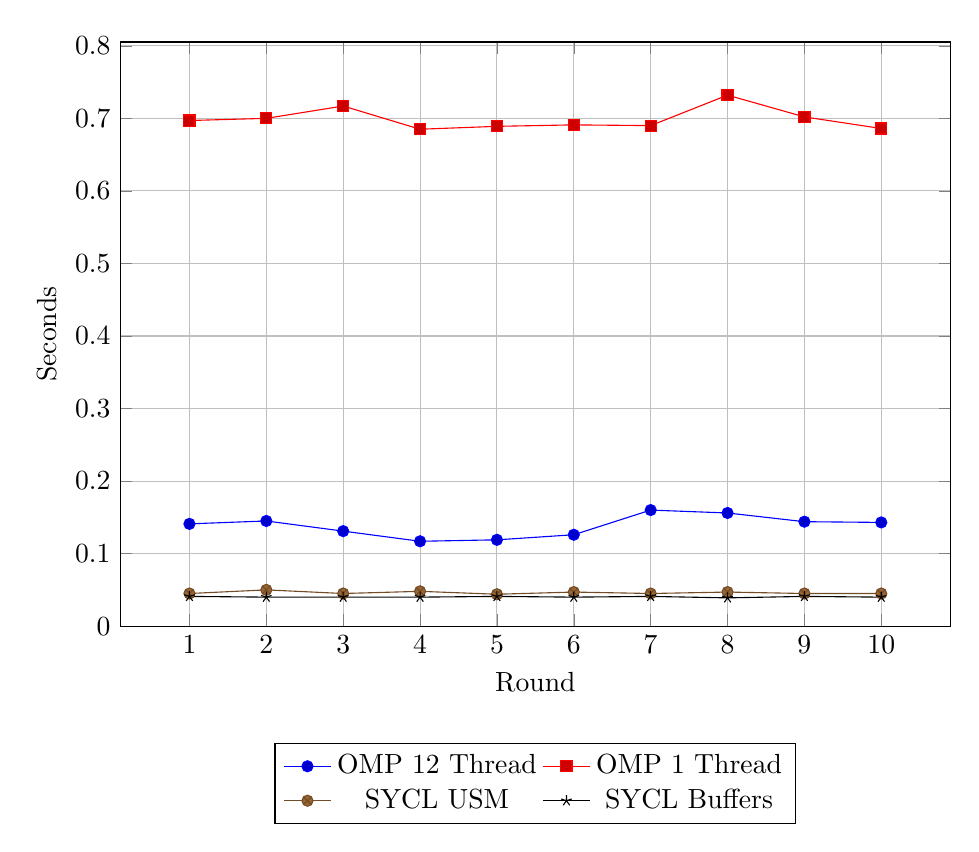
\begin{tikzpicture}
\begin{axis}[
    width=\linewidth,
    height=9cm,
    xlabel={Round},
    ylabel={Seconds},
    legend style={at={(0.5,-0.2)},anchor=north,legend columns=2},
    grid=both,
    ymin=0,
]
\addplot coordinates {
    (1,0.141) (2,0.145) (3,0.131) (4,0.117) (5,0.119)
    (6,0.126) (7,0.160) (8,0.156) (9,0.144) (10,0.143)
};
\addlegendentry{OMP 12 Thread}
\addplot coordinates {
    (1,0.697) (2,0.700) (3,0.717) (4,0.685) (5,0.689)
    (6,0.691) (7,0.690) (8,0.732) (9,0.702) (10,0.686)
};
\addlegendentry{OMP 1 Thread}
\addplot coordinates {
    (1,0.045) (2,0.050) (3,0.045) (4,0.048) (5,0.044)
    (6,0.047) (7,0.045) (8,0.047) (9,0.045) (10,0.045)
};
\addlegendentry{SYCL USM}
\addplot coordinates {
    (1,0.041) (2,0.040) (3,0.040) (4,0.040) (5,0.041)
    (6,0.040) (7,0.041) (8,0.039) (9,0.041) (10,0.040)
};
\addlegendentry{SYCL Buffers}
\end{axis}
\end{tikzpicture}
\caption{Matrix Multiplication Timing Across Implementations ($1000x1000^2$, Release Mode \texttt{-O2}), excluding JIT warmup run.}
\label{fig:timing_graph}
\end{figure}

\subsection{Neural Network}
\par The neural network had two metrics to keep track of: the runtime and the model performance. Both were successfully optimized but were lacking in some ways which are described below. Additionally, further testing should be performed on other datasets to make sure results found here are not anomalies from the dataset's characteristics.
\par The choice to use C++ and prioritize parallelization was an important one if wider datasets are ever attempted on the API. While matrix multiplication parallelization provided the largest gains on large matrices (as shown above), for the relatively small weight matrices in the thyroid dataset, batch-level parallelization proved more impactful, reducing runtime by ~40\%, compared to a theoretical maximum of 50\%, with just two threads. This challenges the proposal presented earlier, but more testing should be performed on higher feature count datasets. The more likely issue is that the size of any matrices being multiplied were too small to give enough work to the thread performing the operation. This may not overcome the overhead of the thread creation in the first place. Here is a graph visualizing the difference in runtime for the methods of parallelization tested: 

\begin{figure}[H]
\centering
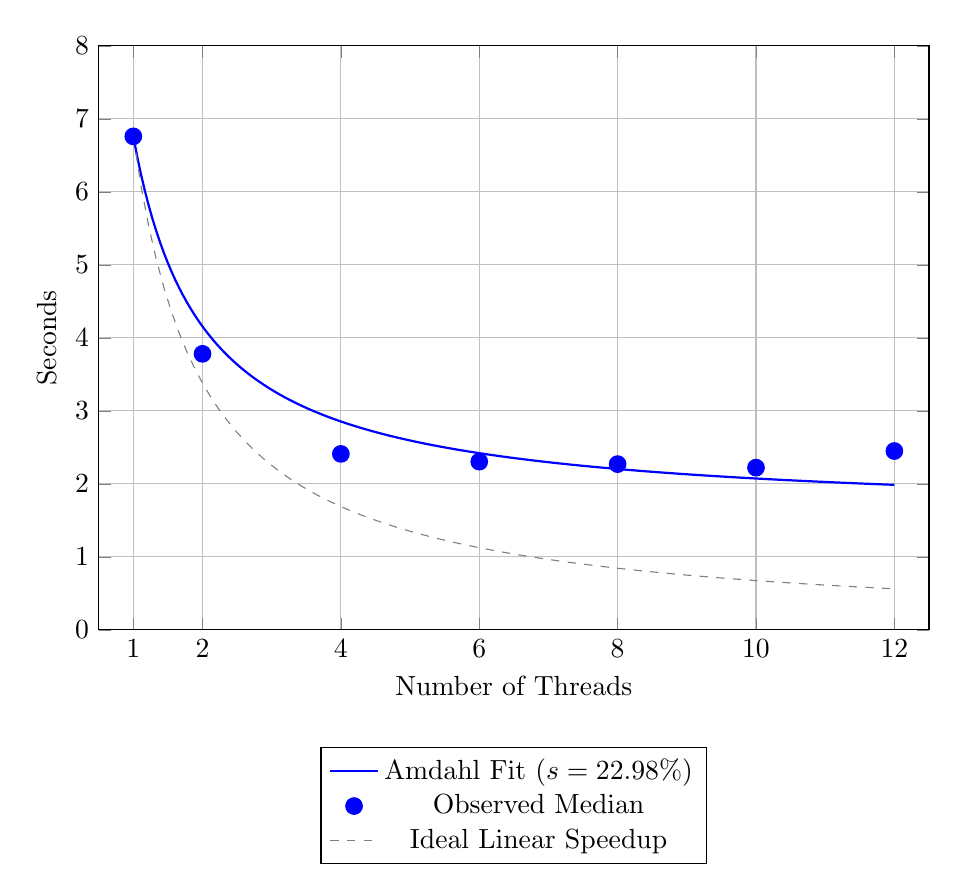
\begin{tikzpicture}
\begin{axis}[
    width=\linewidth,
    height=9cm,
    xlabel={Number of Threads},
    ylabel={Seconds},
    legend style={at={(0.5,-0.2)},anchor=north,legend columns=1},
    grid=both,
    xtick={1,2,4,6,8,10,12},
    xmin=0.5, xmax=12.5,
    ymin=0, ymax=8,
]

% Amdahl fit: T(n) = 6.75974 * (0.2298 + (1-0.2298)/n)
\addplot[
    color=blue,
    thick,
    domain=1:12,
    samples=200,
] {6.75974 * (0.2298 + 0.7702 / x)};
\addlegendentry{Amdahl Fit ($s = 22.98\%$)}

% Observed median points
\addplot[
    color=blue,
    mark=*,
    mark size=3pt,
    only marks,
] coordinates {
    (1,6.75974) (2,3.78153) (4,2.41092) (6,2.304995) (8,2.27095) (10,2.222585) (12,2.450175)
};
\addlegendentry{Observed Median}

% Ideal linear speedup
\addplot[
    color=gray,
    dashed,
    domain=1:12,
    samples=100,
] {6.75974 / x};
\addlegendentry{Ideal Linear Speedup}

\end{axis}
\end{tikzpicture}
\caption{Neural Network Training Time vs.\ Number of OMP Threads, with Amdahl's Law fit ($s = 22.98\%$ serial fraction, max theoretical speedup $= 4.35\times$) and ideal linear speedup shown for reference.}
\label{fig:amdahl_scaling}
\end{figure}

\par Amdahl's Law describes the theoretical speedup of a parallel program as a function of the number of processors and the proportion of the program that must remain serial. Let $T_1$ denote the execution time on a single thread, $n$ the number of threads, and $s \in [0, 1]$ the serial fraction of the program - the portion that cannot be parallelized. The predicted runtime on $n$ threads is given by: 

\begin{equation}
    T(n) = T_1 \left( s + \frac{1 - s}{n} \right)
    \label{eq:amdahl_time}
\end{equation}

The corresponding speedup $S(n)$, defined as the ratio of single-thread runtime to $n$-thread runtime, is:
 
\begin{equation}
    S(n) = \frac{T_1}{T(n)} = \frac{1}{s + \frac{1-s}{n}}
    \label{eq:amdahl_speedup}
\end{equation}
 
As $n \to \infty$, the parallel portion $\frac{1-s}{n} \to 0$, and the speedup approaches a finite upper bound determined entirely by the serial fraction:
 
\begin{equation}
    S_{\max} = \lim_{n \to \infty} S(n) = \frac{1}{s}
    \label{eq:amdahl_max}
\end{equation}
 
The serial fraction $s$ can be estimated empirically by fitting Equation~\ref{eq:amdahl_time} to observed runtimes across multiple thread counts using least squares minimization. In this work, the fitted serial fraction was found to be $s \approx 0.2298$, yielding a theoretical maximum speedup of:

\begin{equation}
    S_{\max} = \frac{1}{0.2298} \approx 4.35\times
    \label{eq:amdahl_max_observed}
\end{equation}

This indicates that approximately $22.98\%$ of the training loop is serial in its current state, imposing a ceiling on parallel efficiency as threads increase. This could be improved by increasing the batch size or restructuring the job allocation again.
\par However, in order to utilize GPU architectures, simply moving an Open MP pragma will not work. In fact, GPU offloading requires minimizing communication between the host device and GPU for meaningful performance increases. Programs utilizing GPU speedups require intentional design around the highly parallel architecture, including minimizing memory use, complex operations, and swaps between devices.
\par A useful comparison for this neural network implementation is the industry standard for machine learning prototyping - PyTorch. By setting up a neural network with the same hyper-parameters and dataset as the one being used with the custom implementation, runtime can be measured. PyTorch can be installed to target both CPU and GPU, for this example the CPU optimized package is installed and trained ten times and training times are measured. 
\par After comparing the runtimes between the custom and PyTorch implementation, PyTorch is faster than the single threaded custom version. However, even after setting the thread count for PyTorch from 1 to 12, the runtime did not improve. This is likely due to the parallelization strategy utilized by the PyTorch team. In fact, the size of the dataset may be why the PyTorch implementation is slower. So, more testing should be done on both implementations across several high cost datasets. However, when the custom neural network parallelization strategy is applied, runtime improves enough to beat the PyTorch model by nearly half the runtime in this case.
\par Both implementations comfortably met the five minute training constraint, and both produced non-trivial classification results on the thyroid dataset. The precision, recall, and F1 scores for the custom implementation are reported in Appendix B.

\section{Limitations}
\subsection{Matrix Multiplication}
\par Due to the way the program is designed to distribute jobs, the performance begins to degrade as the dimensions of the arrays become less square. If the number of rows of the first is too large, the number of jobs will increase dramatically as the work per thread decreases. And the reverse is true for increasingly smaller rows of $a$. Additionally, as any other dimension increases, the work per thread increases dramatically. This can result in reduced performance with awkwardly sized matrix multiplication.
\par Additionally, increasing any dimension of the arrays by ten beyond two 1000 x 1000 matrices will cause at least a ten times increased runtime since there are ten times as many operations to complete and even more data management which could cause cache thrashing. If sufficient resources are unavailable, the program may fail to execute entirely. There are some more memory management optimizations that could be made in the future to prevent at least this part of the issue.
\subsection{Neural Network}
\par Another relevant issue discovered in both the matrix multiplication research and the neural network is the thread synchronization/creation overhead which cannot be overcome in small matrix multiplication such as the Thyroid dataset model. A batch based scheduling algorithm was more successful for this application. Although, more complicated datasets and larger layers within the model could benefit more from the parallel matrix multiplication backend. 
\par Class imbalance presented a separate structural challenge. Without class weighting and the Adam optimizer, the model collapsed to predicting the majority/heaviest class exclusively. This will become more of an issue as the network backend is not optimized to handle other matrix operations in parallel. 
\par Another scalability concern comes in the form of GPU level parallelism. In fact, a restructuring of the entire matrix class would be required to reduce the transfer of matrices between the host device and the GPU.

\section{Future Work}
\par The most immediate priority is extending the neural network backend 
to support GPU acceleration. As noted in the limitations, this requires 
restructuring the matrix class around device-resident memory to minimize 
host-to-device transfers — simply substituting the OpenMP pragma with a 
SYCL kernel will not produce meaningful speedups. Once this is in place, 
the two-level parallelism strategy explored here maps naturally onto 
distributed GPU training: a coordinator distributes batches across 
machines, and each machine further parallelizes individual matrix 
operations across threads or GPU cores. This is the architecture 
underlying large-scale deep learning training today, and this project's 
design is intentionally structured to grow toward it.
\par Portability also remains an open problem. SYCL does not support 
NVIDIA GPUs out of the box, since NVIDIA hardware requires CUDA code to 
function. Codeplay provides a CUDA backend for SYCL that would resolve 
this, though the plugin repository has been intermittently unavailable. 
A promising alternative is AdaptiveCpp, formerly HipSYCL, a 
community-driven open-source compiler that targets NVIDIA, AMD, and Intel 
hardware from a single SYCL compiler. [3] Either path would allow this 
implementation to run on common hardware without vendor-specific 
rewrites, which is the core portability goal.
\par Additionally, the backend modularity would allow different parallel backends to be swapped out dynamically. Including a more optimized matrix implementation potentially allocating matrices on the GPU and only transferring when needed to the CPU. This would allow all matrix operations to be accelerated with parallel structuring and reduce communication overhead. 
\par Finally, the benchmarks presented here warrant a more controlled 
follow-up. The OpenMP and SYCL implementations were compiled with 
different compilers, and compiler optimizations were left at default 
settings for both. A fair comparison would require a unified 
compiler toolchain. While compiler optimizations were flagged to the release level (-O2), the different compilers could have significantly different optimizations in the machine code. These variables were acceptable for an exploratory benchmark but should be addressed before drawing stronger performance conclusions.

\section{Conclusion}
\par Ultimately, parallel programming and its importance will only grow 
from here as humans continually work toward big ideas such as deep 
learning, cloud computing, and lower latency. Using tools such as SYCL 
or other open standards allows developers to fully realize the potential 
of parallel processing.
\par But, optimizations such as employing the correct memory management 
and job distribution strategy are vital to ensuring performant code is 
written with these frameworks. In this implementation, massive speedups 
were achieved with one change alone. Although limitations in portability 
exist now, the infrastructure exists to expand to many different devices.
\par The neural network optimization is just one example of how 
intentional design can result in incredible feats of computing. Software 
developers that learn to build their program around parallel architecture 
will benefit 'linearly'.
\par This project began by establishing that memory model and 
parallelization design are the two decisions that matter most in 
parallel matrix multiplication — demonstrated through a SYCL USM 
implementation that outperformed a 12-thread OpenMP baseline by more 
than three times. That finding then shaped the neural network API, where 
batch-level parallelism proved more effective than fine-grained matrix 
loop parallelism for small weight matrices. Taken together, the results 
argue that workload size must inform parallelization strategy at every 
level of a program's design — from a single kernel to a full training 
loop.
\par In summary, this project demonstrates both the practical performance 
gains achievable through intelligent parallel optimization, the 
real-world applications of these optimizations, and the future of 
portable frameworks to create a more connected device ecosystem. As 
hardware continues to evolve toward greater distributed and parallel 
architecture, these tools will become essential for staying relevant as 
developers. The results from this project represent one step in 
furthering efficient and portable parallel computing.

\appendices
\section{Raw Matrix Multiplication Runtime Data}
Table I presents the raw execution times for multiplying two 1000 x 1000 matrices with random double values on ten timed rounds with the C++ chrono library on a Ryzen 5 9600X CPU. Median, standard deviation, and first and third quartiles were computed and included for reference. A warm up iteration was included for each test to ensure SYCL queue initialization and CPU cache warming did not bias the measured rounds.

\begin{table}[H]
\centering
{\fontsize{14}{16}\selectfont
\resizebox{\linewidth}{!}{
\begin{tabular}{lcccc}
\hline
\textbf{\#} & 
\textbf{SYCL USM} & 
\textbf{12-Thread OMP} &
\textbf{SYCL Buffers} &
\textbf{1-Thread OMP} \\
\hline
0* & 1.363 & 0.141 & 0.404 & 0.697 \\
1  & 0.045 & 0.145 & 0.041 & 0.700 \\
2  & 0.050 & 0.131 & 0.040 & 0.717 \\
3  & 0.045 & 0.117 & 0.040 & 0.685 \\
4  & 0.048 & 0.119 & 0.040 & 0.689 \\
5  & 0.044 & 0.126 & 0.041 & 0.691 \\
6  & 0.047 & 0.160 & 0.040 & 0.690 \\
7  & 0.045 & 0.156 & 0.041 & 0.732 \\
8  & 0.047 & 0.144 & 0.041 & 0.702 \\
9  & 0.045 & 0.143 & 0.039 & 0.686 \\
\hline
\textbf{Std Dev} & 0.041 & 0.015 & 0.006 & 0.015 \\
\textbf{Median}  & 0.046 & 0.142 & 0.041 & 0.694 \\
\textbf{Lower}   & 0.045 & 0.126 & 0.039 & 0.686 \\
\textbf{Upper}   & 0.050 & 0.156 & 0.041 & 0.717 \\
\hline
\end{tabular}
}}
\caption{Execution Times (Seconds) for $1000x1000$ Matrix Multiplication Across Different Implementations (Release Mode, \texttt{-O2})}
\end{table}

The SYCL USM and Buffer implementations were consistently the fastest, with a median runtime of ~0.0435 seconds. Compared to 0.142 seconds for Open MP (12 thread).

\ifCLASSOPTIONcaptionsoff
  \newpage
\fi

\section{Raw Neural Network Performance Data}
Tables II and III present the raw training times and final model evaluation results for the neural network trained on the UCI thyroid dataset. Training times were recorded across ten trials comparing single-threaded and twelve-thread OpenMP execution. The confusion matrix reflects the model's classification performance across three thyroid condition classes on the full dataset.

\begin{table}[H]
\centering
{\fontsize{14}{16}\selectfont
\resizebox{\linewidth}{!}{
\begin{tabular}{lccc}
\hline
\textbf{\#} & 
\textbf{OMP 1 Thread} & 
\textbf{OMP 12 Thread} &
\textbf{Pytorch}\\
\hline
1  & 6.693 & 2.552 & 4.62 \\
2  & 6.809 & 2.472 & 4.62 \\
3  & 7.045 & 2.611 & 4.69 \\
4  & 6.940 & 2.656 & 4.78 \\
5  & 6.782 & 2.473 & 4.64 \\
6  & 6.696 & 2.388 & 4.59 \\
7  & 6.711 & 2.408 & 4.59 \\
8  & 6.755 & 2.413 & 4.7 \\
9  & 6.765 & 2.429 & 4.56 \\
10 & 6.745 & 2.160 & 4.58 \\
\hline
\textbf{Std Dev}    & 0.114 & 0.138 & 0.064 \\
\textbf{Median}     & 6.760 & 2.450 & 4.62 \\
\textbf{Q1 (Lower)} & 6.711 & 2.408 & 4.59\\
\textbf{Q3 (Upper)} & 6.809 & 2.552 & 4.678\\
\hline
\end{tabular}
}}
\caption{Neural Network Training Times (Seconds) Across Implementations}
\end{table}

Median times across ten trials were calculated for thread counts from 1 - 12 as well. The increase in median runtime at 12 threads can be attributed to thread synchronization overhead:

\begin{table}[H]
\centering
{\fontsize{14}{16}\selectfont
\resizebox{\linewidth}{!}{
\begin{tabular}{lccc}
\hline
\textbf{T} &
\textbf{Median Runtime (s)} &
\textbf{Speedup} &
\textbf{Amdahl Predicted (s)} \\
\hline
1  & 6.760 & 1.000$\times$ & 6.760 \\
2  & 3.782 & 1.788$\times$ & 4.157 \\
4  & 2.411 & 2.804$\times$ & 2.855 \\
6  & 2.305 & 2.933$\times$ & 2.421 \\
8  & 2.271 & 2.977$\times$ & 2.204 \\
10 & 2.223 & 3.041$\times$ & 2.074 \\
12 & 2.450 & 2.759$\times$ & 1.987 \\
\hline
\end{tabular}
}}
\caption{Median Neural Network Training Times by Thread Count, with observed speedup relative to 1 thread and Amdahl's Law predicted time ($s = 22.98\%$ serial fraction).}
\end{table}

Additionally, Table IV contains a confusion matrix showing the non-trivial predictions produced by the neural network. Precision, recall, and F1 score have been calculated from this in Table V: 

\begin{table}[H]
\centering
{\fontsize{14}{16}\selectfont
\resizebox{0.95\linewidth}{!}{
\begin{tabular}{lcccc}
\hline
 & \textbf{Pred. Class 1} & \textbf{Pred. Class 2} & \textbf{Pred. Class 3} & \textbf{Total} \\
\hline
\textbf{Actual Class 1} & 66  & 7   & 0    & 73   \\
\textbf{Actual Class 2} & 0   & 163 & 14   & 177  \\
\textbf{Actual Class 3} & 12  & 17  & 1471 & 1500 \\
\hline
\end{tabular}
}}
\caption{Confusion Matrix — UCI Thyroid Dataset Classification Results}
\end{table}

\begin{table}[H]
\centering
{\fontsize{14}{16}\selectfont
\resizebox{\linewidth}{!}{
\begin{tabular}{lcccccc}
\hline
\textbf{Metric} & 
\textbf{Class 1} & 
\textbf{Class 2} & 
\textbf{Class 3} & 
\textbf{Macro Avg} &
\textbf{Weighted Avg} \\
\hline
\textbf{Precision} & 0.846 & 0.872 & 0.991 & 0.903 & 0.973 \\
\textbf{Recall}    & 0.904 & 0.921 & 0.981 & 0.935 & 0.971 \\
\textbf{F1 Score}  & 0.874 & 0.896 & 0.986 & 0.918 & 0.972 \\
\hline
\textbf{Support}   & 73    & 177   & 1500  & —     & 1750  \\
\hline
\end{tabular}
}}
\caption{Per-Class and Aggregate Classification Metrics — UCI Thyroid Dataset}
\end{table}

\section{Acknowledgment}
The author would like to thank Muhammed J. Al-Muhammed and Asim Chaudhry for guidance and feedback throughout this project.

\begin{thebibliography}{1}

\bibitem{}“SYCL 2020 Specification.” The Khronos SYCL Working Group, Nov. 7, 2025 
\bibitem{}“Intel - OneAPI - Programming Guide - Optimize Your SYCL Applications.” Intel, Mar. 31, 2025 
\bibitem{}A. Ozeritskiy, D.-C. Timothée, and M. J. Solanki, “Documentation,” ADAPTIVECPP documentation, https://adaptivecpp.github.io/AdaptiveCpp/ (accessed Apr. 20, 2026).
\bibitem{}R. Quinlan. "Thyroid Disease," UCI Machine Learning Repository, 1986. [Online]. Available: https://doi.org/10.24432/C5D010.
\bibitem{}B. Johnston, J. S. Vetter, and J. Milthorpe, ``Evaluating the 
Performance and Portability of Contemporary SYCL Implementations,'' 
\textit{2020 IEEE/ACM International Workshop on Performance, Portability 
and Productivity in HPC (P3HPC)}, GA, USA, 2020, pp. 45--56, 
doi: 10.1109/P3HPC51967.2020.00010.
\bibitem{}T. G. Mattson, ``How Good is OpenMP,'' 
\textit{Scientific Programming}, vol. 11, no. 2, 
pp. 81--93, 2003, doi: 10.1155/2003/124373.

\end{thebibliography}

\end{document}


